
% ----------------------------------------------------------------------
%  Set the document class
% ----------------------------------------------------------------------
\documentclass[11pt,a4paper,twoside]{article}

% ----------------------------------------------------------------------
% Define external packages, language, margins, fonts and new commands
% ----------------------------------------------------------------------
%\input{preamble} 
\usepackage[utf8]{inputenc}   % <<<<< Linux
\usepackage[english]{babel} % <<<<< English
\usepackage{notoccite}
\usepackage[skip=0.5\baselineskip]{caption}
\hyphenation{GTKWave}
\usepackage{listings}
\usepackage[all]{nowidow}

%blind text
\usepackage{lipsum}

\usepackage{graphicx}
\graphicspath{{./}{../../figlib/}{../mat/}{../sim/}}
\def\FontLn{% 16 pt normal
  \usefont{T1}{phv}{m}{n}\fontsize{16pt}{16pt}\selectfont}
\def\FontLb{% 16 pt bold
  \usefont{T1}{phv}{b}{n}\fontsize{16pt}{16pt}\selectfont}
\def\FontMn{% 14 pt normal
  \usefont{T1}{phv}{m}{n}\fontsize{14pt}{14pt}\selectfont}
\def\FontMb{% 14 pt bold
  \usefont{T1}{phv}{b}{n}\fontsize{14pt}{14pt}\selectfont}
\def\FontSn{% 12 pt normal
  \usefont{T1}{phv}{m}{n}\fontsize{12pt}{12pt}\selectfont}

% Use Arial font as default
%
\renewcommand{\rmdefault}{phv}
\renewcommand{\sfdefault}{phv}
\usepackage{geometry}	
\geometry{verbose,tmargin=2.5cm,bmargin=2.5cm,lmargin=2.5cm,rmargin=2.5cm}

%\usepackage{setspace}
%\renewcommand{\baselinestretch}{1.5}

\usepackage[pdftex]{hyperref} % enhance documents that are to be
                              % output as HTML and PDF
\hypersetup{colorlinks,       % color text of links and anchors,
                              % eliminates borders around links
%            linkcolor=red,    % color for normal internal links
            linkcolor=black,  % color for normal internal links
            anchorcolor=black,% color for anchor text
%            citecolor=green,  % color for bibliographical citations
            citecolor=black,  % color for bibliographical citations
%            filecolor=magenta,% color for URLs which open local files
            filecolor=black,  % color for URLs which open local files
%            menucolor=red,    % color for Acrobat menu items
            menucolor=black,  % color for Acrobat menu items
%            pagecolor=red,    % color for links to other pages
            pagecolor=black,  % color for links to other pages
%            urlcolor=cyan,    % color for linked URLs
            urlcolor=black,   % color for linked URLs
	          bookmarks=true,         % create PDF bookmarks
	          bookmarksopen=false,    % don't expand bookmarks
	          bookmarksnumbered=true, % number bookmarks
	          pdftitle={report},
            pdfauthor={Andre C. Marta},
%            pdfsubject={Thesis Title},
%            pdfkeywords={Thesis Keywords},
            pdfstartview=FitV,
            pdfdisplaydoctitle=true}

\usepackage[numbers,sort&compress]{natbib} % <<<<< References in numbered list [1],[2],...
\usepackage{subcaption} 
\usepackage{mdframed}

%%%%%%%%%%%%%%%%%%%%%%%%%%%%%%%%%%%%%%%%%%%%%%%%%%%%%%%%%%%%%%%%%%%%%%%%
%     Begin Document                                                   %
%%%%%%%%%%%%%%%%%%%%%%%%%%%%%%%%%%%%%%%%%%%%%%%%%%%%%%%%%%%%%%%%%%%%%%%%


\begin{document}

% Set plain page style (no headers, footer with centered page number)
\pagestyle{plain}

% Set roman numbering (i,ii,...) before the start of chapters
%\pagenumbering{roman}

% ----------------------------------------------------------------------
%  Cover page
% ----------------------------------------------------------------------
\thispagestyle {empty}
\includegraphics[bb=9.5cm 11cm 0cm 0cm,scale=0.29]{IST_A_CMYK_POS}
\begin{center}
\vspace{1.0cm}
{\FontLb Circuit Theory and Electronics Fundamentals} 
\vspace{1cm}
{MEAer}
\vspace{1cm}
{\FontSn Example Laboratory Report}
\vspace{1cm}
{\FontSn March 25, 2021}
\end{center}


% ----------------------------------------------------------------------
% Dedication page (optional)
% ----------------------------------------------------------------------
%\input{dedication} 
%\cleardoublepage

% ----------------------------------------------------------------------
%  Acknowledgments (optional)
% ----------------------------------------------------------------------
%\input{acknowledgements}
%\cleardoublepage

% ----------------------------------------------------------------------
%  Abstract (both in English and Portuguese)
% ----------------------------------------------------------------------
%\input{resumo} 
%\cleardoublepage

%\input{abstract} 

% ----------------------------------------------------------------------
%  Table of contents, list of tables, list of figures and nomenclature
% ----------------------------------------------------------------------

% Table of contents
%
\tableofcontents

% List of tables
%\addcontentsline{toc}{section}{\listtablename}
%\listoftables
%\cleardoublepage 

% List of figures
%\addcontentsline{toc}{section}{\listfigurename}
%\listoffigures
%\cleardoublepage 

% Set arabic numbering (1,2,...) after preface
%
%\setcounter{page}{1}
%\pagenumbering{arabic}

% ----------------------------------------------------------------------
%  Body
% ----------------------------------------------------------------------

\section{Introduction}
\label{sec:Introduction}

The objective of this laboratoty is to study the behaviour of the circuit using nodal method and mesh method.The curcuit contains both dependent and independent current and voltage source, $I_b$,$I_d$,$V_c$ and $V_a$ respectively.The circuit also has resistors with known resistance.The circuit can be seen in figure~\ref{fig:rc} .



In Section~\ref{sec:analysis}, a theoretical analysis of the circuit is
presented. In Section~\ref{sec:simulation}, the circuit is analysed by
simulation, and the results are compared to the theoretical results obtained in
Section~\ref{sec:analysis}. The conclusions of this study are outlined in
Section~\ref{sec:conclusion}.

\begin{figure}[h] \centering
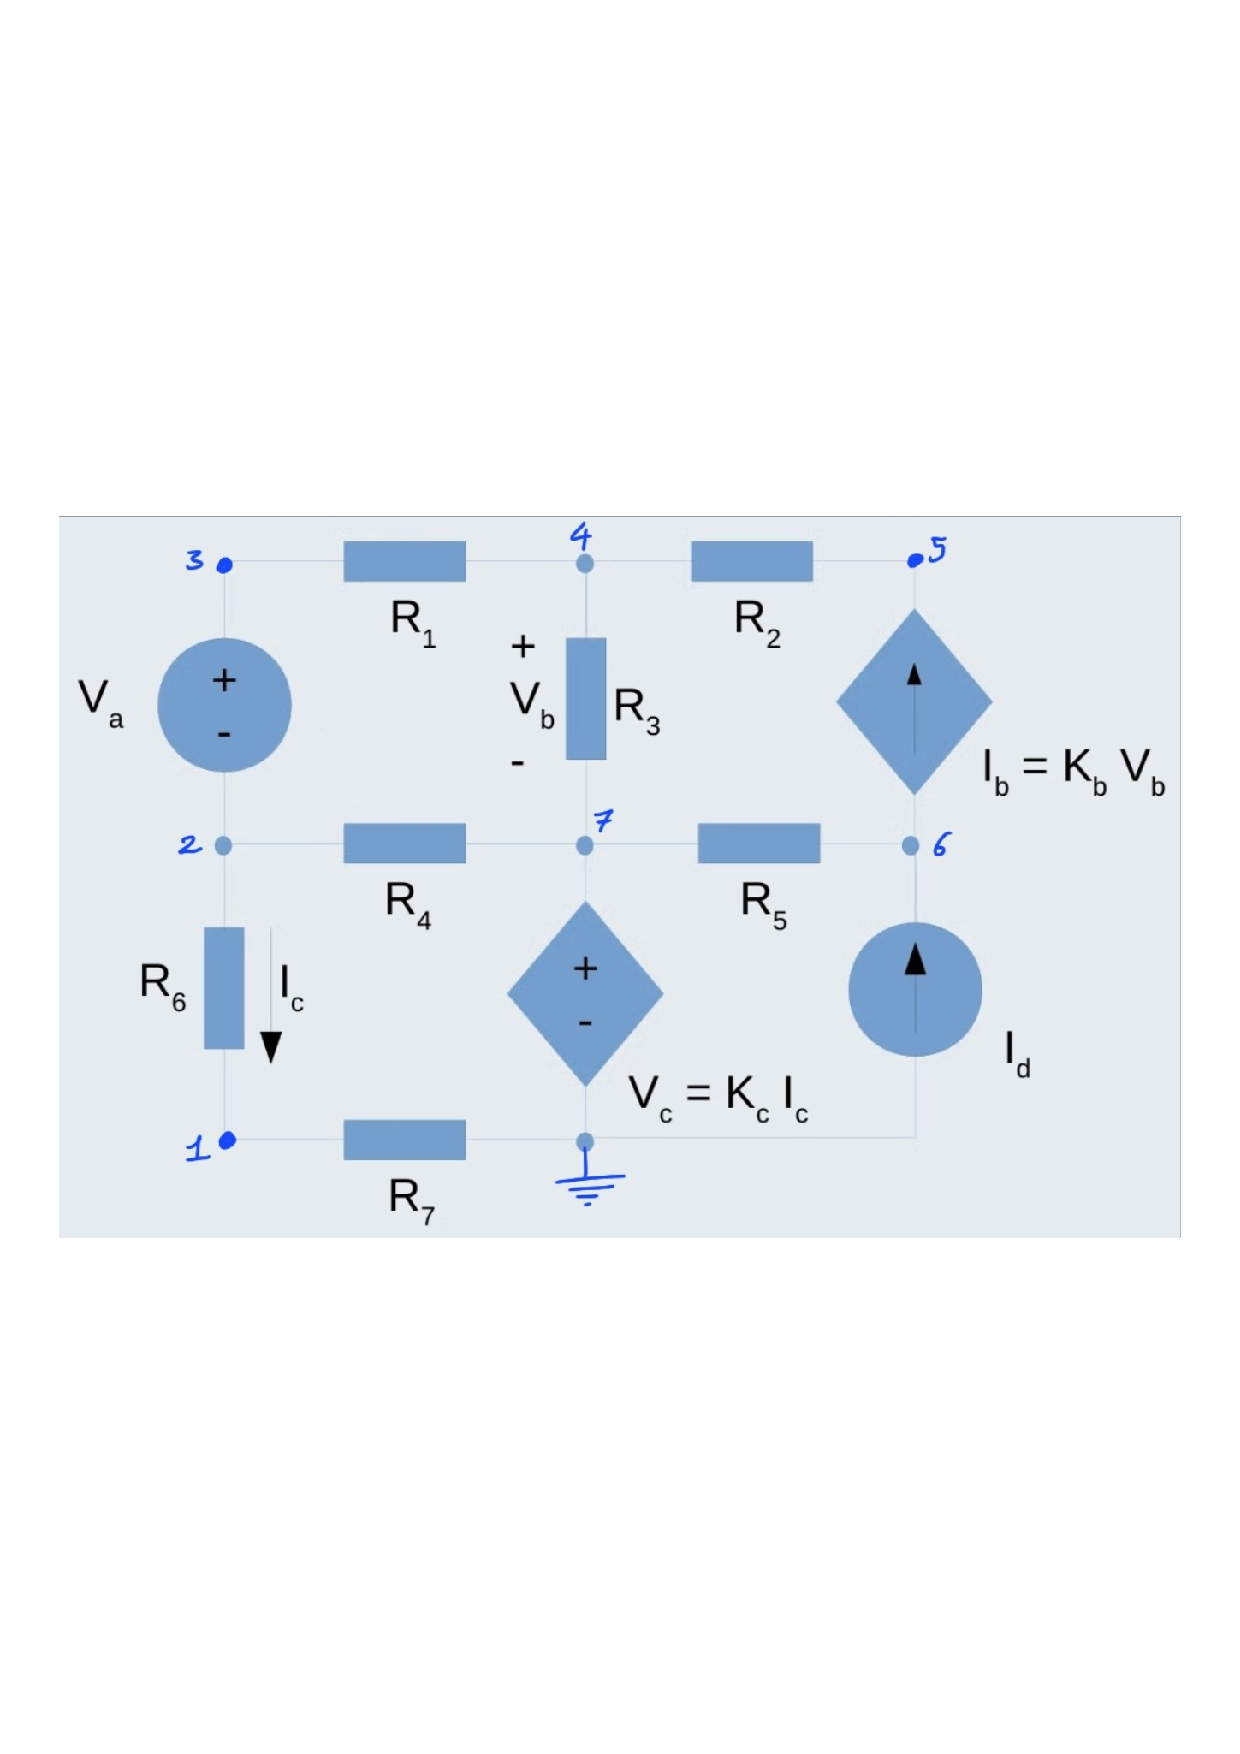
\includegraphics[width=0.4\linewidth]{rc}
\caption{Dependent and Independent sources circuit.}
\label{fig:rc}
\end{figure}



\section{Theoretical Analysis}
\label{sec:analysis}
This section, the circuit shown in Figure 1 is analysed
theoretically, in terms of nodal and mesh method.

\subsection{Nodal method}

$R_1=1.0216234171$

$R_2=3.0213296603$

$R_4=4.17287588373$

$R_5=3.07453996538$

$R_6=2.06761158432$

$R_7=7.0023872588$

$I_d=1.00202530449$

$K_b=1.00202530449$

$K_c=8.38330387808$


The circuit has $7$ nodes,labeled as $1$ to $7$.Node $0$ is chosen as ground($V_0=0$).Using KCL for essential nodes(node 1,4,5,and 6),we have:


Node 1: $\frac{V_1}{R_7}+\frac{V_2-V_1}{R_6}$

Using conductance, $G=\frac{1}{R}$, we get:

$V_1G_7+(V_2-V_1)-G_6$.....................................................(1)

Node 4:

$(V_3-V_4)G_1-(V_4-V_7)G_3+(V_5-V_4)G_2$..................................(2)

Node 5:

$I_b=(V_5-V_4)G_2$..........................................................(3)

Node 6:

$I_d-I_b=(V_6-V_7)G_5$.......................................................(4)

For node 7, $V_7=V_c=K_cI_c$


Using octave to find the nodes voltages we get:

$V_1=C_3$\\

$V_4=\frac{G_3C_3+I_b}{G_1+G_3}$\\


$V_5=\frac{G_2G_3C_3+I_b(G_1+G_2+G_3)}{G_2(G_1+G_3)}$\\


$V_6=C_3+\frac{I_d}{G_5}$

Substituting with the known values we have:

$V_1=3.02$\\

$C_3+3.0745=V_b$\\

$V_6=6.09$\\

$0.68C_3+I_b=V_5$\\

$0.68(3.02)+I_b=V_5$\\

$V_5=2.05+I_b$\\

$0.25(C_3+I_b)=V_4$\\

$0.25(3.02+I_b)=V_4$\\

$0.76+0.76I_b=V_4$\\

$\frac{-V_5-V_4}{R_2}+I_b$\\


$\frac{-2.05-I_b0.76-0.76I_b}{2.01}=-I_b$\\


$\frac{-2.70I_b-0.76}{2.01}=-I_b$\\


$-2.70I_b-0.76=-2.01I_b$\\

$0.69I_b=0.76$\\

$I_b=-1.10mA$\\

$V_5=2.05-1.10$\\

$V_5=0.95v$\\

$V_4=-0.076v$\\

$V_4=0.076v$\\

$V_6=6.09V$\\

$V_1=3.02v$


\subsection{Mesh method}

Using KVL to find the currents in a circuit in Figure~\ref{---------},we have:

Mesh 1:

$I_1=-I_b=-K_bV_b$..............................................................(1)

Mesh 2:

$I_2=-I_d$.......................................................................(2)

Mesh 3:

$-I_3(R_7+R_6+R_4)+R_4-I_4=V_c$..................................................(3)

Mesh 4:

$I_1R_3+I_3R_4-I_4(R_1+R_3+R_4)=-V_a$

Using octave we get the values of currents as:

$I_1=-I_b$\\

$I_2=I_d$\\

$I_3=\frac{I_bR-3R_4-R_4V_a+V_c(R_1+R_3+R_4)}{R_4^2-(R_1+R_3+R_4)(R_4+R_6+R_7}$\\


$I_4=\frac{I_bR_3(R_4+R_6+R_7)+R_4V_c-V_a(R_4+R_6+R_7)}{R_4^2-(R_1+R_3+R_4)(R_4+R_6+R_7}$\\

Sustituting and doing algebra we get values I as:

$I_1=1.10mA$\\
$I_2=1mA$\\
$I_3=0.65mA$\\
$I_4=1.44mA$\\

Current that is flowing in each resister is:\\

$I_{R_1}=1.44mA$\\
$I_{R_2}=1.00mA$\\
$I_{R_3}=0.34mA$\\
$I_{R_4}=0.79mA$\\
$I_{R_5}=0.1mA$\\
$I_{R_6}=0.65mA$\\
$I_{R_7}=0.65$\\




%\section{Simulation}

\label{sec:simulation}

\subsection{Operating Point Analysis}

Table~\ref{tab:op} shows the simulated operating point results for the circuit
under analysis. Compared to the theoretical analysis results, one notices the
following differences:

\begin{table}[h]
  \centering
  \begin{tabular}{|l|r|}
    \hline    
    {\bf Name} & {\bf Value [mA and V]} \\ \hline
    @gb[i] & -1.68378e-01\\ \hline
@id[current] & 1.000000e+00\\ \hline
@r1[i] & -1.68378e-01\\ \hline
@r2[i] & -1.68378e-01\\ \hline
@r4[i] & -2.66153e-01\\ \hline
@r5[i] & -1.16838e+00\\ \hline
@r6[i] & -9.77754e-02\\ \hline
@r7[i] & -9.77754e-02\\ \hline
a & -5.41101e+00\\ \hline
b & -5.31323e+00\\ \hline
c & -5.10986e+00\\ \hline
d & 1.201401e-01\\ \hline
e & -5.16055e-02\\ \hline
f & -3.90045e-01\\ \hline
g & -4.13079e-01\\ \hline
h & -4.00000e+00\\ \hline

  \end{tabular}
  \caption{Operating point. A variable preceded by @ is of type {\em current}
    and expressed in mA; other variables are of type {\it voltage} and expressed in
    Volt.}
  \label{tab:op}
\end{table}

\lipsum[1-1]



%\section{Conclusion}
\label{sec:conclusion}

In this laboratory assignment the objective of analysing the circuit has been
achieved. Voltage and currents of resistors have been performed both
theoretically using the Octave maths tool and by circuit simulation using the
Ngspice tool. The simulation results does not matched the theoretical results
precisely. The reason for this may be due to the errors been made during theoretical analysis when doing algebra and computing the equations.

\lipsum[1-1]

%\cleardoublepage

% ----------------------------------------------------------------------
%  Bibliography
% ----------------------------------------------------------------------
%\addcontentsline{toc}{section}{\bibname}
%\bibliographystyle{abbrvunsrtnat} % <<<<< SELECT IF USING REFERENCES BY NUMBER (CITATION ORDER)
%\bibliography{../../../BIBfile.bib}

% ----------------------------------------------------------------------
\end{document}
% ----------------------------------------------------------------------
